\documentclass[16pt]{beamer}
\usepackage[utf8]{inputenc}

\title{Les données personnelles}

\usetheme{default}

\usepackage[utf8]{inputenc}
\usepackage{amsmath}
\usepackage{amsfonts}
\usepackage{amssymb}
\usepackage{pgf}
\usepackage{color}
\usepackage[frenchb]{babel}
\usepackage{amssymb}
\usepackage{hyperref}

\usefonttheme{default}
\usepackage{DejaVuSans}
%\usepackage[sfdefault]{FiraSans} %% option 'sfdefault' activates Fira Sans as the default text font
\usepackage[T1]{fontenc}
\renewcommand*\oldstylenums[1]{{\firaoldstyle #1}}


\setbeamertemplate{navigation symbols}{} %remove navigation symbols

\author{Cédric Jeanneret (aka \href{https://www.twitter.com/SwissTengu}{@SwissTengu})}
\institute{\href{https://www.ethack.org/}{EthACK.org}}
\date{\today}

\definecolor{linecolor}{HTML}{4d4c4c}

\setbeamercolor{linecolor}{fg=white,bg=linecolor}

\setbeamertemplate{headline} {
	\begin{beamercolorbox}[wd=\paperwidth,dp=8pt,ht=12pt,leftskip=.29cm,rightskip=.29cm]{linecolor}
	\hfill
	\hypersetup{
		colorlinks=true,
		linkcolor=white,
		urlcolor=white,
	}
	\insertinstitute
	\end{beamercolorbox}%
}

\setbeamertemplate{footline}{%
	\begin{beamercolorbox}[wd=\paperwidth,dp=9pt,ht=0.4cm,leftskip=.29cm,rightskip=.3cm]{linecolor}
	\pgfputat{\pgfxy(0.455,-0.315)}{\pgfbox[center,base]{
\includegraphics[width=1.5cm]{../common/logo_537.png}}}
	\hfill
	\inserttitle
	\end{beamercolorbox}%
}


\hypersetup{
	colorlinks=true,
	linkcolor=blue,
	urlcolor=blue,
	pdfborderstyle={/S/U/W 1},
	pdfborder=0 0 1,
	linkbordercolor={0 0 0},
	urlbordercolor={0 0 0},
}


\begin{document}

{
\setbeamertemplate{footline}{%
	\begin{beamercolorbox}[wd=\paperwidth,dp=8pt,ht=12pt,leftskip=.29cm,rightskip=.3cm]{linecolor}
	\hfill
	\inserttitle
	\end{beamercolorbox}%
}

% center first slide — not a title, but almost
{
\centering
\begin{frame}

EthACK
\vspace{0.5cm}

The Swiss Privacy Basecamp 
\vspace{0.5cm}


\includegraphics[width=4cm]{../common/logo_537.png}

\end{frame}
}
}

\begin{frame}{EthACK ?}
\begin{itemize}
	\item Éthique
	\item État
	\item ACKnowledgement (reconnaissance)
	\item Hacking (éthique, évidemment)
	\item …
\end{itemize}
\end{frame}

\begin{frame}{Pourquoi ?}
\begin{itemize}
	\item Notre gouvernement ne s'intéresse pas (ou peu) au sujet
	\item Les sociétés privées nous fichent à notre insu
	\item Personne ne sait où sont leurs données, qui les traitent, à quoi elles servent
\end{itemize}
\end{frame}


\begin{frame}
  \titlepage
\end{frame}

\begin{frame}
{Contenu de la présentation}
\begin{itemize}
\item Un peu de légal
\item Un peu d'exemples
\item Hygiène des nuages
\item E-Health, est-ce hygiénique ?
\end{itemize}
\end{frame}

\begin{frame}
{La loi fédérale}
RS235.1, article 3 : \newline
On entend par: \newline
a. données personnelles (données), toutes les
informations qui se rapportent à une personne
identifiée ou identifiable;
\end{frame}

\begin{frame}
{RS235.1, art 3}
On entend par : \newline
b. personne concernée, la personne physique ou morale au sujet de laquelle des données sont traitées;
\end{frame}

\begin{frame}
{RS235.1, art 3}
On entend par : \newline
c. données sensibles, les données personnelles sur:
\begin{itemize}
\item les opinions ou activités religieuses, philosophiques, politiques ou syndicales,
\item la santé, la sphère intime ou l'appartenance à une race,
\item des mesures d'aide sociale,
\item des poursuites ou sanctions pénales et administratives;
\end{itemize}
\end{frame}

\begin{frame}
{Loi complète}
\begin{figure}

\includegraphics[height=3cm,keepaspectratio]{./qrcode-lpd.png} \newline
\end{figure}
\begin{center}
\href{http://www.admin.ch/opc/fr/classified-compilation/19920153/index.html}{Loi fédérale sur la protection des données}
\end{center}
\end{frame}

\begin{frame}
{Fin du légal ;)}
\begin{figure}

\includegraphics[height=3cm,keepaspectratio]{./boringclass_Large.jpg}
\end{figure}
\end{frame}

\begin{frame}
{Exemple de données}
\begin{itemize}
\item Nom, dettes, adresse, email, téléphone
\item Prénom, état civil, casier judiciaire, numéro AVS
\item Nom des parents, des enfants, du conjoint, poursuites
\end{itemize}
\end{frame}

\begin{frame}
{Exemple de données… Sensibles !}
\begin{itemize}
\item Nom, \textbf{dettes}, adresse, email, téléphone
\item Prénom, état civil, \textbf{casier judiciaire}, numéro AVS
\item Nom des parents, des enfants, du conjoint, \textbf{poursuites}
\end{itemize}
\end{frame}

\begin{frame}
{De l'utilité de ces données}
\begin{itemize}
\item Elles nous définissent en tant qu'individu
\item Elles nous démarquent de la masse
\end{itemize}
\begin{center}
\textbf{Certaines sont utilisées pour des décisions qui nous concernent}
\end{center}
\end{frame}

\begin{frame}
{Des décisions ?}
\begin{itemize}
\item La \textbf{gérance} de votre appartement sera intéressée par vos \textit{dettes}, \textit{poursuites} et \textit{salaire}.
\item Un nouvel \textbf{employeur} peut être intéressé par votre \textit{casier judiciaire} ou votre \textit{dossier médical}.
\item Votre \textbf{assureur} sera intéressé par votre \textit{dossier médical}.
\end{itemize}
\end{frame}

\begin{frame}
{Hmmm…}
\begin{figure}

\includegraphics[height=3cm,keepaspectratio]{./suspicious.png}
\end{figure}
\end{frame}

\begin{frame}
{Collect}
\begin{itemize}
\item Par l'État.
\item Par des sociétés privées.
\end{itemize}
\vspace{1cm}
\begin{itemize}
\item Depuis le pays d'habitation.
\item Depuis l'étranger.
\end{itemize}
\end{frame}

\begin{frame}
{Qui en profite ?}
\begin{itemize}
\item L'État
\item Les entreprises privées
\item En tous cas pas vous \newline
{\tiny à moins que vous n'aimiez la publicité ciblée, entre autre…}
\end{itemize}
\end{frame}

\begin{frame}
{Un marché}
On achète des données comme on achète du pain.\newline
\vspace{1cm}

{«Marché noir» : le propriétaire légitime (VOUS) ne sait rien de ce commerce…}
\end{frame}

\begin{frame}
{Pourquoi se protéger ?}
\begin{itemize}
\item Vous ne savez pas qui possède des données sur vous
\item Vous ne savez pas quelles données ils possèdent
\item Vous ne savez pas ce qu'ils en font
\end{itemize}
\end{frame}

\begin{frame}
{Et alors ?!}
\begin{center}
«Je n'ai rien à cacher de toutes façons !»
\end{center}
\end{frame}

\begin{frame}
{Et alors ?!}
\begin{center}
«Je n'ai rien à cacher de toutes façons !»\newline
\vspace{0.5cm}

(Ministre du IIIème Reich à l'Éducation du peuple et à la Propagande — Joseph Goebbels)\newline
\vspace{0.5cm}

\textit{Vous n'avez rien à craindre si vous n'avez rien à cacher.}
\end{center}
\begin{figure}
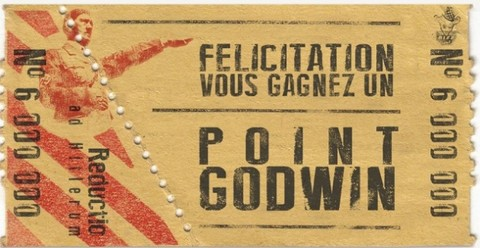
\includegraphics[height=1.5cm,keepaspectratio]{./Point-Godwin_univers-grande.jpg}
\end{figure}
\end{frame}

\begin{frame}
{Pourquoi se protéger ?}
\begin{itemize}
\item Vous ne savez pas si les données sont à jour
\end{itemize}
\vspace{0.5cm}
\begin{itemize}
\item Des {\color{red}décisions capitales} pour vous peuvent être prises sans que vous ne sachiez pourquoi.
\item Ces décisions peuvent être basées sur des {\color{red}données erronées ou dépassées}.
\end{itemize}
\end{frame}

\begin{frame}
{Exemples}
\begin{itemize}
\item Un {\color{red}crédit peut vous être refusé} sans que vous ne sachiez pourquoi
\item Un {\color{red}logement peut vous être refusé} sans que vous ne sachiez pourquoi
\end{itemize}
\begin{figure}

\includegraphics[height=3cm,keepaspectratio]{./frigtened-kitten.jpg}
\end{figure}
\end{frame}

\begin{frame}
{Qui ?}
\begin{itemize}
\item Plus de {\color{red}100} entités privées ont des informations sur {\color{red}vos poursuites}.
\item Plus de {\color{red}250} entités privées ont des informations sur {\color{red}vos revenus}.
\item Plus de {\color{red}170} entités privées ont des informations sur {\color{red}votre situation financière}.
\end{itemize}
\tiny{Source: \href{https://www.datareg.admin.ch/WebDatareg/search/search.aspx?lang=fr}{Registre des fichiers}}
\end{frame}

\begin{frame}
{Qui ? (bis)}
\begin{itemize}
\item Plus de {\color{red}300} entités privées ont des données sur {\color{red}votre santé}.
\item Environ {\color{red}50} entités privées ont des informations sur {\color{red}votre origine}.
\item Environ {\color{red}50} entités privées ont des informations sur {\color{red}votre religion}.
\end{itemize}
\tiny{Source: \href{https://www.datareg.admin.ch/WebDatareg/search/search.aspx?lang=fr}{Registre des fichiers}}
\end{frame}

\begin{frame}
{Pourquoi ?}
Les motifs varient beaucoup
\begin{itemize}
\item Services après-vente
\item Ciblage publicitaire
\item Profilage (officieusement)
\item «Prises de décisions» diverses
\begin{itemize}
\item Crédit
\item logement
\item …
\end{itemize}
\item …
\end{itemize}
\end{frame}

\begin{frame}
{Pourquoi ? (bis)}
\begin{itemize}
\item Protection de la population
\begin{itemize}
\item Police (les vilains pédonazis tueurs de chatons)
\item Terrorisme
\item Hooligans
\item …
\end{itemize}
\end{itemize}
\end{frame}

\begin{frame}
{Le Cloud}
\begin{center}
\large Un nuage de données personnelles
\end{center}
\end{frame}

\begin{frame}
{Pourquoi l'employer ?}
\begin{itemize}
\item Sauvegardes.
\item Accès aux données depuis partout.
\item Accès via son smartphone.
\item … et encore tant de raisons.
\end{itemize}
\begin{center}
En gros, c'est pratique ;)
\end{center}
\end{frame}

\begin{frame}
{Pourquoi ne pas employer ?}
\begin{itemize}
\item Hébergement sur sol étranger (lois).
\item Sécurité.
\item Complexité pour trier ce qu'on envoie ou non.
\item Certains sont gratuits, mais à quel prix ?
\end{itemize}
\end{frame}

\begin{frame}
{Mais je veux employer !}
\begin{itemize}
\item Garder en tête que c'est online.
\item Garder en tête que, potentiellement, ce n'est JAMAIS effacé.
\item Ne pas mettre de photos compromettantes.
\item Ne pas mettre de documents sensibles.
\end{itemize}
\end{frame}

\begin{frame}
{Hygiène du Cloud}
\begin{itemize}
\item Ce que tu enverras sur le cloud tu trieras.
\item Une confiance limitée tu donneras.
\item Un mot de passe solide tu utiliseras.
\item Une solution avec chiffrement côté client tu privilégieras.
\end{itemize}
\begin{figure}

\includegraphics[height=2cm]{./yoda.jpg}
\end{figure}
\end{frame}

\begin{frame}
{Xaskubmglbml ?!}
\begin{itemize}
\item Chiffrer : action de rendre illisible un document \newline
{\tiny « crypter » dans les médias}
\item Son contraire : déchiffrer \newline
{\tiny Et PAS « décrypter » !}
\end{itemize}
\end{frame}

\begin{frame}
{Chiffrement côté client}
\begin{itemize}
\item Les documents sont chiffrés sur votre appareil avant d'être envoyés.
\item Le service de stockage ne peut pas lire (à priori).
\item Protège des interceptions lors des synchronisation (à priori).
\end{itemize}
\end{frame}

\begin{frame}
{Traqueurs d'activité}
\begin{center}
\large Le nouveau trend du moment
\end{center}
\end{frame}

\begin{frame}
{Principes}
\begin{itemize}
\item Un appareil enregistre vos activités.
\item Il se connecte à Internet.
\item Il envoie toutes les informations collectées.
\end{itemize}
\end{frame}

\begin{frame}
{Problèmes}
\begin{itemize}
\item Vous ne savez pas exactement ce qui est envoyé, ni où
\item Vous partagez des données sensibles avec un tiers privé, situé généralement à l'étranger
\end{itemize}
\end{frame}

\begin{frame}
{Pourquoi est-ce un problème ?}
\begin{itemize}
\item Une société privée basée à l'étranger n'est {\color{red}pas soumise aux lois suisses} sur la protection des données.
\item Une telle société peut faire des accords avec d'autres sociétés.
\end{itemize}
\end{frame}

\begin{frame}
{Pourquoi est-ce un problème ?}
\begin{itemize}
\item Un accord avec un groupe d'assurances, par exemple (voir Apple aux USA).
\item De manière générale, partez du principe que vos données deviennent publiques.
\end{itemize}
\end{frame}

\begin{frame}
{Pourquoi est-ce un problème ?}
\begin{itemize}
\item Vous perdez la vue d'ensemble des accès à ces données (qui, quoi, quand).
\item Certaines données sont clairement du ressort de votre médecin, pas de Google, Apple ou Microsoft (glucose, pression, etc).
\end{itemize}
\end{frame}

\begin{frame}
{Conclusion}
\begin{itemize}
\item Vos données sont précieuses.
\item Il existe un marché pour ces données.
\item Vous n'êtes pas le bénéficiaire principal de ce marché
\item Maintenant que vous en savez un peu plus, réfléchissez avant d'employer des services ;)
\end{itemize}
\end{frame}

{
\setbeamertemplate{footline}{%
	\begin{beamercolorbox}[wd=\paperwidth,dp=8pt,ht=12pt,leftskip=.29cm,rightskip=.3cm]{linecolor}
	\hfill
	\inserttitle
	\end{beamercolorbox}%
}
{
\centering
\begin{frame}
{Questions ?}

\href{https://ethack.org/}{https://ethack.org/} \\
\vspace{0.3cm}
\href{https://www.twitter.com/EthACK_org}{@EthACK\_org} on Twitter \\
\vspace{0.3cm}
\href{https://www.facebook.com/ethack.org}{ethack.org} on Facebook

\vspace{0.5cm}


\includegraphics[width=4cm]{../common/logo_537.png}
\end{frame}
}
}

\end{document}